\section{DFT}

\paragraph{Fourier Transform}
transforms time continuos values in time domain into values in frequency domain.

\(u(t) \laplace \underline{U}(f)=\int_{-\infty}^{+\infty}u(t) \cdot \euler^{-j 2 \pi f t} dt \)

\paragraph{Discrete Fourier Transform} 
is the Fourier Transform for time discrete values.

\( u(kT_s) \laplace  \underline{\tilde{U}}(\frac{n}{N \cdot T_s})= \sum_{k=0}^{N-1} u(kT_s) \cdot \euler^{-j 2 \pi n \frac{k}{N}} \)

with N: number of sampled values \\and \(n = 0, 1, 2, ... , N-1\).

Quantity of must-calculate-values: $\frac{N}{2} + 1$ \figref{fig:mirrorValues}

\begin{figure}
	\centering
	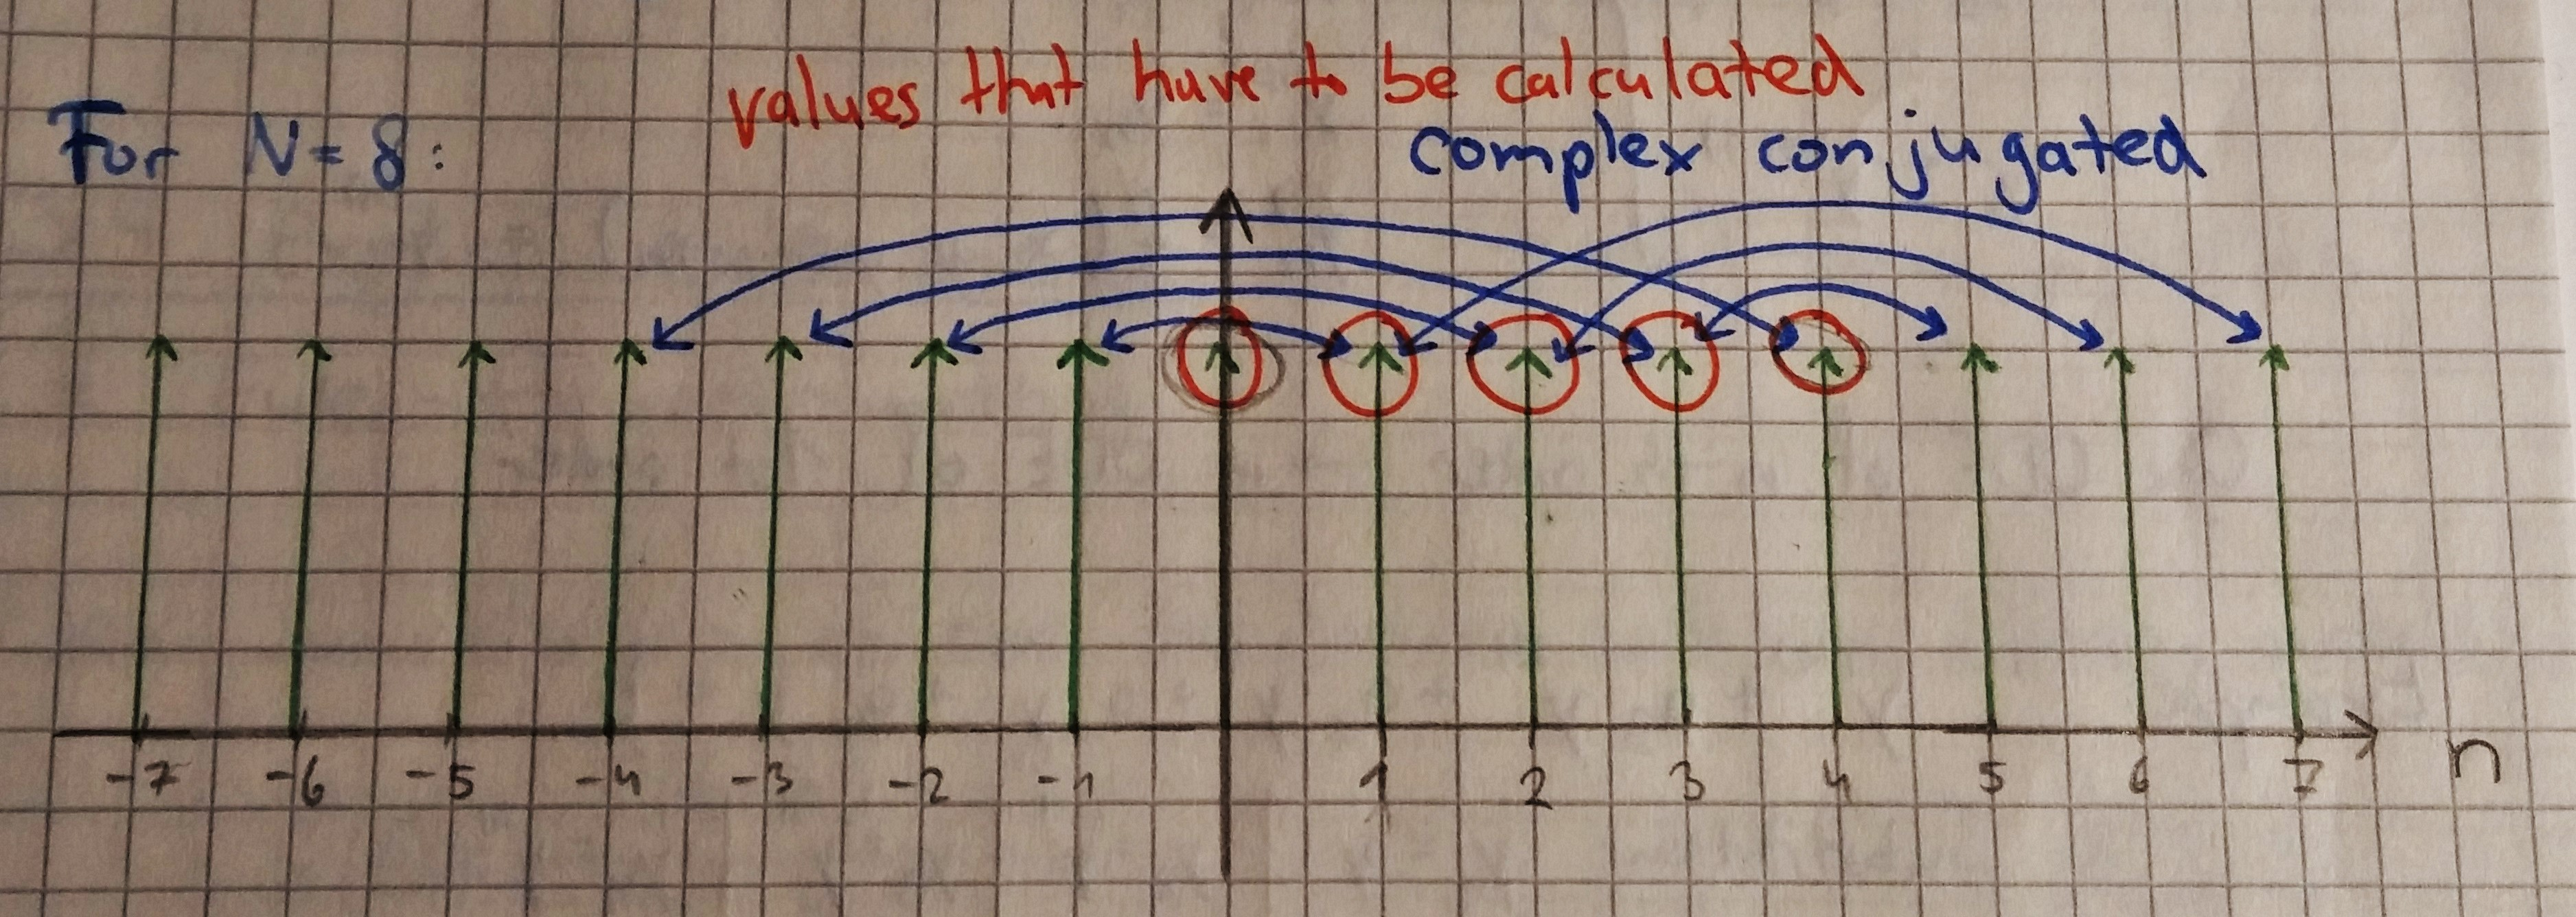
\includegraphics[width=0.9\linewidth]{images_LA/mirrorValues}
	\caption{Complex conjugated values}
	\label{fig:mirrorValues}
\end{figure}

Solution vector for $N=8$:

\(\underline{\tilde{U}}(\frac{n}{N \cdot T_s})= \begin{bmatrix}
\underline{\tilde{U}}(\frac{0}{N \cdot T_s}) \\
\underline{\tilde{U}}(\frac{1}{N \cdot T_s})  \\
\underline{\tilde{U}}(\frac{2}{N \cdot T_s}) \\
\underline{\tilde{U}}(\frac{3}{N \cdot T_s})\\
\underline{\tilde{U}}(\frac{4}{N \cdot T_s})\\
\underline{\tilde{U}}(\frac{5}{N \cdot T_s})\\
\underline{\tilde{U}}(\frac{6}{N \cdot T_s})\\
\underline{\tilde{U}}(\frac{7}{N \cdot T_s})\\
\underline{\tilde{U}}(\frac{8}{N \cdot T_s})\\
\underline{\tilde{U}}(\frac{9}{N \cdot T_s})\\
\vdots 
\end{bmatrix}
\)
=
\(
\begin{matrix}
	\text{just calculate}\\
	\vdots \\
	\vdots \\
	\vdots \\
	\vdots \\
	\text{complex conjugated of } \underline{\tilde{U}}(\frac{3}{N \cdot T_s})\\
	\text{complex conjugated of } \underline{\tilde{U}}(\frac{2}{N \cdot T_s})\\
	\text{complex conjugated of } \underline{\tilde{U}}(\frac{1}{N \cdot T_s})\\
	\underline{\tilde{U}}(\frac{0}{N \cdot T_s})\\
	\underline{\tilde{U}}(\frac{1}{N \cdot T_s})\\
	\vdots 
\end{matrix}
\)

Here you have to calculate \(\frac{8}{2}+1=5\) values (namely $n=0, 1, 2, 3, 4$). from who the other ones (namley $n=5, 6, 7$) can be deduced. The N-th value is the same as $n=0$ because of the periodic repitition. 

\paragraph{Inverse discrete Fourier Transform}
calculates the values in time domain out of the DFT.

\( u(kT_s) = \frac{1}{N} \sum_{n=0}^{N-1} \underline{\tilde{U}}(\frac{n}{N \cdot T_s}) \cdot \euler^{j 2 \pi n \frac{k}{N}} \) 

with \(k = 0, 1, 2, ... , N-1\).
